\section{Nine copper coins, and other toposes}
\epigraph{Explicaron que una cosa es \emph{igualdad}, y otra \emph{identidad}, y formularon una especie de \emph{reductio ad absurdum}, o sea el caso hipotético de nueve hombres que en nueve sucesivas noches padecen un vivo dolor. ¿No sería ridículo -interrogaron- pretender que ese dolor es el mismo?}{JLB ---Tl\"on, Uqbar, Orbis Tertius}
According to our description of the internal language of variable sets, \emph{propositions} in $\Set/I$ are morpisms of the form
\[p : U \to \Omega_I\]

where $\Omega_I$ is the subobject classifier of \ref{}; recall that
\begin{itemize}
  \item the object $\Omega_I = \{0,1\}\times I \to I$ becomes a variable set in a canonical way with the projection $\pi_I : \Omega_I \to I$ on the second factor;
  \item the universal monic $I \to \Omega_I$ consists of a section of $\pi_I$, precisely the one that sends $i : I$ to the pair $(i,1) : \Omega_I$;
  \item every subobject $U \hookrightarrow A$ of an object $A$ results as a pullback (in $\Set/I$) along true:
        \[\xymatrix@R=5mm@C=5mm{
          U\ar[dr]^u\ar[rr]^u\ar[dd]_m&& I\ar[dd]^{\sf t} \ar@{=}[dl]\\
          &I& \\
          A \ar[ur]\ar[rr]_{\chi_U}&& \ar[ul]\Omega_I
        }\]
        (see \ref{} for a complete proof)
\end{itemize}
L'insieme $I$ deve essere pensato in questa prospettiva come a un ``moltiplicatore'', oppure come uno ``sfumatore'' di valori di verità. Introduciamo questa notazione: diciamo che $p : U \to \Omega_I$ è vera (risp., falsa), nel contesto $x :U$, con \emph{forza} $t$ se $p(x) =(1,t)$ (risp., $p(x)=(0,t)$).

So, a proposition is a morphism of the following kind: it is a function $p : U \to \Omega_I$, defined on a certain domain, and such that
\[
\xymatrix{
  U\ar[d]_u\ar[r]^-p  & \{0,1\}\times I \ar[d]^{\pi_I}\\ 
  I \ar@{=}[r]& I
}  
\]
(it must be a morphism of variable sets!) This means that $\pi p(x : U) = u(x : U)$, so that $p(x) = (\epsilon_x, u(x))$ for $\epsilon_x =0,1$ and $u$ is uniquely determined by the "variable domain" $U$. Questa è una osservazione importante perché dice che la ``forza'' con cui $p$ è vera è completamente determinata dalla struttura di $U$ come oggetto di $\Set/I$.

To get a grip dei vari ruoli di diverse classi di proposizioni, e dato che noi ci concentreremo -costruendola ex nihilo- su una classe di proposizioni particolare, è conveniente discutere ora quale struttura $I$ debba avere. In effetti, differenti scelte di $I$ dànno luogo a differenti categorie di insiemi variabili; in ciascuna di queste è possibile esprimere diversi paradossi: l'insieme ``nudo'' $I$  viene equipaggiato con maggior struttura (per esempio una struttura d'ordine o topologica) per dare ai valori di verità analoga maggiore struttura.

Segue roundup di esempi; ciascuno di loro è così organizzato: rammentiamo il paradosso o il passo che vogliamo analizzare; mostriamo in quale topos tale paradosso non è tale, perché si riduce a una sentenza perfettamente lecita, che non ha niente di paradossale nel linguaggio interno degli insiemi variabili, e che appare invece paradossale per gli abitanti della copia di $\Set$ che sta dentro gli insiemi variabili.

Spesso usiamo $I=[0,1]$; ci sono diversi motivi per questa scelta, il più lampante è il seguente: se un valore di verità ora è sempre dato con una certa \emph{forza} $t\in I$; è naturale voler confrontare tra loro gli elementi dell'insieme di queste forze: bisogna essere in grado di asserire quale tra due proposizioni date è vera con forza ``maggiore''. Perciò, anche se questa ipotesi non è mai strettamente necessaria (l'unico vincolo posto da questa condizione naturale è che $I$ sia almeno parzialmente ordinato da una relazione $\le$), una scelta naturale per $I$ lo prende come un continuo (=un insieme totalmente ordinato, denso, ove vale la LUP --cita un libro a caso di descriptive set theory). Una opzione alternativa droppa la densità: in tal caso, l'ordine lineare finito $I=\Delta[n]$, $I=\omega = \bigcup_n \Delta[n]$ sono scelte abbastanza standard. In ciascuno di questi casi la logica classica si recupera come segue\todo{\dots}
\begin{center}
  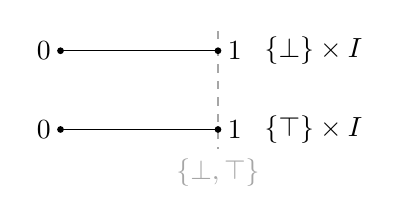
\begin{tikzpicture}
    \draw[gray!70,dashed] (2,1.25) -- (2,-.25) node[below] {$\{\perp,\top\}$};
    \draw[fill] (0,0) circle (1pt) node[left] {$0$};
    \draw[fill] (2,0) circle (1pt) node[right] (dis) {$1$};
    \draw (0,0) -- (2,0);
    \begin{scope}[yshift=1cm]
    \draw[fill] (0,0) circle (1pt) node[left] {$0$};
    \draw[fill] (2,0) circle (1pt) node[right] (dat) {$1$};
    \draw (0,0) -- (2,0);
    \node[right of=dis] {$\{\top\}\times I$};
    \node[right of=dat] {$\{\perp\}\times I$};
    \end{scope}
    \end{tikzpicture}
\end{center}
(sebbene $I$ sia rappresentato come un intervallo, $0$ e $1$ sono solo dei segnaposto per il minimo e massimo di $I$ quando esso sia linearmente ordinato.)
\begin{remark}
  Un esempio interessante è $I=\{0<\frac{1}{2}< 1\}$: $\Omega_I$ in questo caso è l'insieme totalmente ordinato $\Delta[1]\times\Delta[2]$ che si rappresenta pictorialmente come 
  \[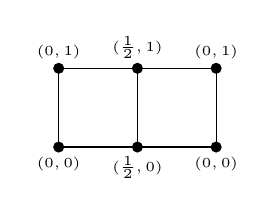
\begin{tikzpicture}[xscale=2]
    \foreach \i/\name in {0/0,.5/{\frac{1}{2}},1/0}{
      \foreach \j/\pos in {0/below,1/above}
        \fill (\i,\j) ellipse (1pt and 2pt) node[\pos] {\tiny $(\name,\j)$};
    }
    \draw (0,0) rectangle (1,1);
    \draw (.5,1) -- (.5,0);
    \end{tikzpicture}\]
  Vi è sempre un minimax, respectively in $(0,0)$ e in o$(1,1)$, ma vi sono elementi non confrontabili tra loro; il risultato è un'algebra i Heyting? Sono gli aperti dello spazio di Sierpinski. Quindi sì, conticino.
  
  In un setting come questo, eventi nello spazio continuo dovrebbero dar luogo a cambi istantanei di stato nella forza del modo in cui sono veri/falsi; è invece ragionevole che la forza con cui $p$ è vera vari continuamente se dipende da variabili continue.\footnote{Il fatto che a rigore tali variazioni continue di valore di verità non avvengano nel nostro mondo è alla base della famiglia di paradossi del \emph{separating instant}: quanto è ben definita la nozione di ``istante del decesso''? Quanto è ben definita la nozione di istante di tempo?}

  Per questo motivo è piu conveniente prendere per $I$ una struttura continua; e prenderla in maniera tale che sia univocamente caratterizzata da queste proprietà. Per esempio possiamo prendere $I=[0,1]$; in \cite{} Freyd caratterizza $I$ come l'oggetto universale con certe proprietà, e bla bla bla. questo dà luogo e avere un poset dei valori di verità; è un poset particolarmente bello: è un frame, quindi anche un'algebra di Heyting $\fkH =([0,1],\land,\lor,\Rightarrow)$ rispetto allo pseudocomplemento dato da $(x \Rightarrow z) := \bigvee_{x\land y \le z} y$ (è infatti immediato verificare che $x \land a \le b$ if and only if $a \le x \Rightarrow b$ per ogni $a,b\in [0,1]$).
\end{remark}
\subsection{The unimaginable topos theory hidden in Borges' library}
\begin{remark}
  Siccome il caso $I=[0,1]$ con la topologia euclidea è quello piu naturale per diversi motivi, definiamo alcuni insiemi di interesse per una data proposizione $p : U \to \Omega_I$ per questa scelta di $I$:
\begin{itemize}
  \item $A^\top = \{x : U \mid p(x) = (1,t_x), t_x > 0\} = p^\leftarrow(\{1\}\times (0,1])$ e $A^\perp = \{x : U \mid p(x) = (0,t_x), t_x > 0\}$; cose vere (risp., false) con forza maggiore di zero. Sono le funzioni $u : U \to I$ tali che $u^\leftarrow 0 = \varnothing$.
  \item $B^\top = \{x : U \mid p(x) = (1,1)\} = p^\leftarrow((1,1))$ e $B^\perp = \{x : U \mid p(x) = (0,1)\}$ cose vere (risp.,false).
  \item $E_t^\top = \{ x : U \mid p(x)=(1,t)\}$ e $E_t^\perp = \{ x : U \mid p(x)=(0,t)\}$; cose vere (risp., false) con forza $t$.
\end{itemize}
\end{remark}
\begin{example}
  la freccia, le monete. Rammentiamo il paradosso da \cite{} 
  \begin{quote}
    El martes, $X$ atraviesa un camino desierto y pierde nueve monedas de cobre.
    El jueves, $Y$ encuentra en el camino cuatro monedas, algo herrumbradas por la
    lluvia del miércoles. El viernes, $Z$ descubre tres monedas en el camino. El viernes
    de mañana, $X$ encuentra dos monedas en el corredor de su casa. El heresiarca
    quería deducir de esa historia la realidad -id est la continuidad- de las nueve
    monedas recuperadas. Es absurdo (afirmaba) imaginar que cuatro de las
    monedas no han existido entre el martes y el jueves, tres entre el martes y la
    tarde del viernes, dos entre el martes y la madrugada del viernes. Es lógico
    pensar que han existido -siquiera de algún modo secreto, de comprensión vedada
    a los hombres- en todos los momentos de esos tres plazos. 
  \end{quote}
  $X$ perde le monete, e la forza con cui esistono si abbassa; cresce, e torna massima, ma non per tutte le monete, quando X le ritrova sul portone,  e $Y$ ne trova altre arrugginite per la pioggia (ma siccome il rame non arrugginisce, non sono arrugginite "a causa" della pioggia: in una sorta di principio di wormhole, eventi indipendenti sulla terra sono dipendenti su Tlön, perché l'evento A influenza, in uno spazio pluridimensionale di scelte di z di verità, l'evento B in modi che gli sarebbero vietati se fosse sulla Terra.) $\Omega_I = \{0<1\}\times I$ dove $I$ è un qualsiasi insieme con più di un elemento; esempio minimale, $I=\{N,S\}$ (suddivisione del mondo, e delle ontologie del mondo, in due emisferi), esempio psicologicamente interessante: $I=[0,1]$ (c'è un continuo non numerabile di forze distinte con cui una proprietà può essere vera o falsa); $[0,1]$ è anche il luogo standard dove interpretare logiche sfumate, sebbene lì in senso probabilistico.
\end{example}
\begin{example}
  la lotteria a Babilonia: proposizioni $p : U \to \Omega_{[0,1]}$ possono essere fortemente discontinue: allora esse descrivono un evento innescato come termine finale di una catena di eventi apparentemente disconnessi e paradossali;\footnote{Assumendo una base reale per lo spazio dei parametri da cui $p$ dipende, la sua dipendenza continua è la seguente proprietà: \dots; ciò significa che eventi vicini --nello spazio o nella consequenzialità-- non possono avere valori di verità diversi} in questo mondo, un modello del quale è probabilmente la Babilonia dei ``sorteggi impersonali, di proposito indefinito'', azioni apparentemente scorrelate tra loro (scagliare ``nelle acque dell'Eufrate uno zaffiro di Taprobana''; sciogliere ``dal tetto d'una torre [\dots\unkern] un uccello''; togliere (o aggiungere) ``un granello di rena ai grani innumerevoli della spiaggia'', hanno ``conseguenze, a volte, tremende''.
\end{example}
\begin{example}
  Per quanto riguarda le proposizioni che sono continue nelle proprie variabili, invece, esempio canonico sono le ``tigri di cristallo'' e le ``torri di sangue'' di Tl\"{o}n: oggetti ed entità usuali, diversi da quelli ``classici'' per un dettaglio solo (il colore, la consistenza, il materiale di cui sono composte). Oppure dipendenti in maniera \emph{monotona} e continua dai loro paramentri: $p$ è tanto più vera quanta più gente la osserva, perché ``Le cose, su Tlön, si duplicano; ma tendono anche a cancellarsi e a  perdere i dettagli quando la gente le dimentichi. È classico l'esempio di  un'antica soglia, che perdurò finchè un mendicante venne a visitarla, e che alla  morte di colui fu perduta di vista. Talvolta pochi uccelli, un cavallo, salvarono le  rovine di un anfiteatro. ''
        \[\textstyle p(\exists\text{rovine dell'anfiteatro}, n) = \big(\top, 1-\frac{1}{n}\big)\]
        se $n$ è il numero di persone che vede l'anfiteatro.
\end{example}
\begin{example}
  Il Berkeley idealista degli infiniti istanti di tempo continuo, disconnessi e incomunicabili: $\Omega_I = \coprod_{t : [0,1]} \{ 0 < 1 \}$. E' evidente come questa struttura logica influenzi il linguaggio: i termini sono costruiti per accrezione istantanea, per somma disgiunta dei costituenti e delle loro proprietà: ``aereo-chiaro sopra scuro rotondo''; oggetti determinati dalla sola simultaneità, più che da una dipendenza logica. Altra conferma di ciò, l'abbandono della consequenzialità temporale sta nel passo ``Spinoza attribuisce alla sua inesauribile divinità i modi del pensiero e dell'estensione; su Tlön, nessuno comprenderebbe la giustapposizione del  secondo (che caratterizza solo alcuni stati) e del primo, che è un sinonimo  perfetto del cosmo. In altre parole: non concepiscono che lo spaziale perduri  nel tempo. La percezione di una fumata all'orizzonte, e poi della campagna  incendiata, e poi della sigaretta mal spenta che provocò l'incendio, è  considerata un esempio di associazione di idee.'' Ciò si lega anche al passo ``L'universo è paragonabile a quelle crittografie in cui non tutti i segni hanno un valore, e che solo è vero ciò che accade ogni trecento notti'': un mondo dove ogni trecento notti $p(x) =(\top,1)$, e per le successive 299 notti $p$ ha forza $<1$.
\end{example}
\begin{example}
  
\end{example}
